\chapter{Variational Inference}
\label{chap:vi}

% --- FALLBACK MACROS TO FIX COMPILATION FAILURES ---
\makeatletter
\providecommand{\N}{\mathcal{N}}
\providecommand{\bvec}[1]{\bm{#1}}
\providecommand{\mat}[1]{\mathbf{#1}}
\providecommand{\R}{\mathbb{R}}
\providecommand{\trace}{\operatorname{tr}}
\providecommand{\x}{\mathbf{x}}
\providecommand{\y}{\mathbf{y}}
\providecommand{\T}{^{\top}}
\providecommand{\UUthetahat}{\mat{U}_{\hat{\bvec{\theta}}}\mat{U}_{\hat{\bvec{\theta}}}\T}
\providecommand{\UUthetahatt}{\mat{U}_{\hat{\bvec{\theta}}^{(t)}}\mat{U}_{\hat{\bvec{\theta}}^{(t)}}\T}
\makeatother
% --- table helpers (make stddev safe in/out of math mode)
\makeatletter
\@ifundefined{stddev}{%
  \newcommand{\stddev}[1]{\ensuremath{\pm #1}}%
}{%
  \renewcommand{\stddev}[1]{\ensuremath{\pm #1}}%
}%
\makeatother
\newcommand{\maybeincludegraphics}[2][]{%
  \IfFileExists{#2}{\includegraphics[#1]{#2}}{\fbox{Missing: #2}}%
}
\providecommand{\brackleft}[1]{\hspace{#1}}
\providecommand{\brackright}[1]{\hspace{#1}}\providecommand{\stddev}[1]{\ensuremath{\pm #1}}
\providecommand{\im}{\textrm{im}}
\providecommand{\ker}{\textrm{ker}}

% Algorithms (for the VIKING pseudocode in Variational_Inference.tex)
\SetCommentSty{emph}
\SetProgSty{textup}
% ---------------------------------------------------

\begin{keypointsbox}
\noindent
\textbf{Key points (Chapter~\ref{chap:vi}).}
\begin{enumerate}\setlength{\itemsep}{2pt}
  \item \textbf{The dataset-restricted model map.}
\end{enumerate}
\end{keypointsbox}

\begin{center}
\begin{minipage}{0.95\linewidth}
\noindent\textbf{Chapter \thechapter\ -- Geometric Computations via Matrix-Free Linear Algebra:}\par\vspace{3pt}

\begin{tabular}{@{}p{0.83\linewidth}r@{}}
\hyperref[sec:bridge_dg_la]{\thechapter.1\;\;From Geometry to Linear Algebra} \dotfill & \pageref{sec:bridge_dg_la}\\
\hyperref[sec:la_computations]{\thechapter.2\;\;Efficient Linear Algebra for Deep Learning} \dotfill & \pageref{sec:la_computations}\\
\end{tabular}
\end{minipage}
\end{center}


\noindent
In the previous chapter, we explored the parameter space geometry of models in Bayesian Deep Learning.
However, to accomplish anything of practical significance, we need to be able to compute geometric quantities on this manifold.
At first inspection, this task might seem completely hopeless. The parameter space is a $D$-dimensional manifold, where $D$ is the number of parameters, which can be at the order of billions.
However, as we will show in this chapter, the decomposition of the tangent space of the manifold into the kernel and image can make various computations tractable.
In this chapter, we will begin with a brief recap of the parameter space geometry derived from the previous chapter.
We will then proceed to show how this geometry affects the computation of various geometric quantities that live on this manifold, and finally, how they mostly translate to well-known linear algebra problems.
Finally, we will develop linear algebra algorithms that can scale to large models.

\section{VIKING: \underline{V}ariational \underline{I}nference with \underline{K}ernel- and \underline{I}mage-spaces of \underline{n}umerical \underline{G}auss--Newton matrices}
\label{sec:kivi}
We next build a variational training loop designed with overparametrization in mind.
We start from the ever-present prior $p(\bvec{\theta}) = \N(\bvec{\theta} | \vec{0}, \alpha^{\scriptscriptstyle{-1}} \mathbb{I})$ over parameters $\bvec{\theta} \in \R^D$, with precision $\alpha \in \R$.
As motivated earlier, we choose a variational family $q(\bvec{\theta})$ that is linked to the kernel of an empirical estimate of the Fisher--Rao (FR) metric at $\hat{\bvec{\theta}}$, denoted $\ker(\mathcal{F}_{\hat{\bvec{\theta}}}) \subset \R^D$.
Specifically,
\begin{align}
  \label{eq:approximate-posterior}
  q(\bvec{\theta}) = \N(\bvec{\theta} | \hat{\bvec{\theta}}, \mat{\Sigma}_{\hat{\bvec{\theta}}}) 
  , \quad
    \mat{\Sigma}_{\hat{\bvec{\theta}}}    = \sigma_{\ker}^2 \UUthetahat + \sigma_{\im}^2 (\mathbb{I} - \UUthetahat).
\end{align}
Here, $\mat{U}_{\hat{\bvec{\theta}}} \in \R^{D \times R}$ is a $R$-dimensional basis of the kernel, such that $\UUthetahat$ is a projection matrix that maps parameter vectors in $\R^D$ to the linear subspace $\ker(\mathcal{F}_{\hat{\bvec{\theta}}})$.
In other words, for any $\vec{v} \in \R^D$ we have $\UUthetahat \vec{v} \in \ker(\mathcal{F}_{\hat{\bvec{\theta}}})$, wherein the model's loss is unchanged at the data used to estimate the FR.
\looseness=-1

This proposed approximate posterior is perhaps the simplest possible choice that is adapted to overparametrized models: it has one scalar parameter, $\sigma_{\im}^2 \in \R_+$, that influences the predictive uncertainty on the training data, and another scalar parameter $\sigma_{\ker}^2 \in \R_+$ that reflects uncertainty elsewhere.
Arguably, it is overly simplistic to calibrate a neural network through two scalars, but we will see that it is surprisingly competitive, suggesting that explicitly reflecting overparametrization is important in Bayesian approximations.

\begin{algorithm}[t]
  \caption{The VIKING algorithm}
  \label{alg:viking}
  \begin{algorithmic}[1]
  \REQUIRE Initial values of $(\hat{\bvec{\theta}}, \sigma_{\ker}, \sigma_{\im})$, dataset with $B$ mini-batches
  \ENSURE Optimized values of $(\hat{\bvec{\theta}}, \sigma_{\ker}, \sigma_{\im})$, representing $q(\bvec{\theta})$ (\Cref{eq:approximate-posterior})
  \FOR{each epoch}
    \FOR{each Monte Carlo sample $s = 1$ to $S$}
      \STATE Take $\bvec{\epsilon}^{(s, 0)} \sim \mathcal{N}(\vec{0}, \mathbb{I})$
      \FOR{each mini-batch $t = 1$ to $B$}
        \STATE Compute $\bvec{\epsilon}^{(s, t)}$ from $\bvec{\epsilon}^{(s, t-1)}$ (\Cref{eq:normaleq-initial}) \COMMENT{Alternating projections}
      \ENDFOR
      \STATE $\bvec{\epsilon}_{\ker}^{(s, 0)} \gets \bvec{\epsilon}^{(s, B)}$
    \ENDFOR
    \FOR{each mini-batch $t = 1$ to $B$}
      \FOR{each Monte Carlo sample $s = 1$ to $S$}
        \STATE Compute $\bvec{\epsilon}_{\ker}^{(s, t)}$ from $\bvec{\epsilon}_{\ker}^{(s, t-1)}$ (\Cref{eq:altproj-process})
        \STATE $\bvec{\epsilon}_{\im}^{(s, t)} \gets \bvec{\epsilon}^{(s, 0)} - \bvec{\epsilon}_{\ker}^{(s, t)}$
        \STATE $\bvec{\theta}^{(s)} \gets \hat{\bvec{\theta}} + \sigma_{\ker} \bvec{\epsilon}_{\ker}^{(s, t)} + \sigma_{\im} \bvec{\epsilon}_{\im}^{(s, t)}$ \COMMENT{A sample from $q(\bvec{\theta})$}
      \ENDFOR
      \STATE $\hat{\bvec{\theta}}, \sigma_{\ker}, \sigma_{\im} \gets $ Gradient step on $\mathcal{L}(\hat{\bvec{\theta}}, \sigma_{\ker}, \sigma_{\im})$ using $\{ \bvec{\theta}^{(s)} \}_{s=1}^S$ (\Cref{eq:elbo})
    \ENDFOR
  \ENDFOR
  \end{algorithmic}
\end{algorithm}

\subsection{The VIKING ELBO}

To estimate $q(\bvec{\theta})$, we maximize the usual (variational) lower bound $\mathcal{L}$ of the likelihood $p(\vec{y} | \bvec{\theta}, \x)$
\begin{align}
  \label{eq:elbo}
  \mathcal{L}(\hat{\bvec{\theta}}, \sigma_{\ker}, \sigma_{\im})
    &= \mathbb{E}_{\bvec{\theta} \sim q}\left[ \log p(\y | \bvec{\theta}, \x) \right]
     - \mathrm{KL}( q(\bvec{\theta}) \| p(\bvec{\theta}) ),
\end{align}
where $\mathrm{KL}$ denotes the Kullback-Leibler divergence.
We call the result \emph{Variational Inference with Kernel- and Image-spaces of numerical Gauss--Newton matrices (VIKING)}.
The overall algorithmic steps involved in our method are summarized in \Cref{alg:viking}.
We refer to the two terms of the ELBO as the \emph{reconstruction term} and the \emph{KL term}, respectively, and discuss their evaluation in what follows.

\paragraph{The reconstruction term.}
Assume access to an algorithm to approximate products between the projection matrix $\UUthetahat$ and any vector $\vec{v} \in \R^D$.
For $s = 1, \ldots, S$, we can then estimate of the reconstruction term as
\begin{align}
  \bvec{\epsilon}^{(s)}   &\sim \N(0, \mathbb{I})
                   & \in \R^D, \\
  \text{(projection onto kernel space)} \quad
  \bvec{\epsilon}_{\ker}^{(s)} &= \UUthetahat \bvec{\epsilon}^{(s)}
                   & \in \R^D, \label{eq:kernel-projection}\\
  \text{(image space is orthogonal)} \quad
  \bvec{\epsilon}_{\im}^{(s)} &= (\mathbb{I} - \UUthetahat) \bvec{\epsilon}^{(s)} = \bvec{\epsilon}^{(s)} - \bvec{\epsilon}_{\ker}^{(s)}
                   & \in \R^D, \\
  \bvec{\theta}^{(s)}     &= \hat{\bvec{\theta}} + \sigma_{\ker} \bvec{\epsilon}_{\ker}^{(s)} + \sigma_{\im} \bvec{\epsilon}_{\im}^{(s)}
                   & \in \R^D, \\
  \mathbb{E}_{\bvec{\theta} \sim q}\left[ \log p(\y | \bvec{\theta}, \x) \right]
                   &\approx \frac{1}{S} \sum_{s=1}^S \log p(\y | \bvec{\theta}^{(s)}, \x)
                   & \in \R\phantom{^D} \label{eq:elbo-expectation}.
\end{align}
Here, \Cref{eq:kernel-projection} requires careful computation, to be addressed later.
Once $\bvec{\epsilon}_{\ker}^{(s)}$ is computed, obtaining a sample $\bvec{\theta}^{(s)}$ from the approximate posterior is trivial.

\paragraph{The KL term.}
Since we have both a Gaussian prior and a Gaussian approximate posterior, we can evaluate the KL term in closed form with
\begin{align}
  \label{eq:elbo-kl}
  \mathrm{KL}( q(\bvec{\theta}) \| p(\bvec{\theta}) )
    &= \frac{1}{2} \left( \alpha  \trace(\mat{\Sigma}_{\hat{\bvec{\theta}}}) - D + \alpha \|\hat{\bvec{\theta}}\|^2 - D \log(\alpha) - \log\det(\mat{\Sigma}_{\hat{\bvec{\theta}}}) \right).
\end{align}
Recall the construction of $\mat{\Sigma}_{\hat{\bvec{\theta}}}$ from \Cref{eq:approximate-posterior}.
Since $\mat{\Sigma}_{\hat{\bvec{\theta}}}$ is a sum of scaled projection matrices, it has $R$ eigenvalues equal to $\sigma_{\ker}^2$ and $D\!-\!R$ eigenvalues equal to $\sigma_{\im}^2$.
We can, thus, evaluate
\begin{align}
  \label{eq:trSigma}
  \trace(\mat{\Sigma}_{\hat{\bvec{\theta}}})   &= \sigma_{\ker}^2 R + \sigma_{\im}^2 (D\!-\!R), \text{ and} \\
  \log\det(\mat{\Sigma}_{\hat{\bvec{\theta}}}) &= 2 R \log(\sigma_{\ker}) + 2(D\!-\!R) \log(\sigma_{\im}),
\end{align}
requiring only an estimate of the kernel dimension $R$ to evaluate the full KL term in closed form.
To estimate $R$, we note that $\UUthetahat$ is a projection matrix, i.e., it has $R$ eigenvalues that are 1 while the remaining are 0. Consequently,
\begin{align}
  R = \trace(\UUthetahat)
    \approx \frac{1}{S} \sum_{s=1}^S {\bvec{\epsilon}^{(s)}}\T \overbrace{\UUthetahat \bvec{\epsilon}^{(s)}}
    = \frac{1}{S} \sum_{s=1}^S  {\bvec{\epsilon}^{(s)}}\T \bvec{\epsilon}_{\ker}^{(s)},
\end{align}
where the approximation is Hutchinson's trace estimator \citep{hutchinson1989stochastic}. Note that we may reuse $\bvec{\epsilon}_{\ker}^{(s)}$ (\Cref{eq:kernel-projection}) from the reconstruction term.

\subsection{Kernel projections}\label{sec:kernel-projections}
At first glance, the ELBO terms (\Cref{eq:elbo-expectation,eq:elbo-kl}) seem straightforward.
The practical difficulty lies in projecting onto $\ker(\mathcal{F}_{\hat{\bvec{\theta}}})$ as per \Cref{eq:kernel-projection}.
One noticeable challenge is $\UUthetahat$ having $D \!\times\!D$ entries, where $D$ is the number of model parameters.
With many modern models having millions or billions of parameters, it is not possible to instantiate this matrix, and we resort to matrix-free algorithms.

We start by defining the matrix containing a stack of \emph{per-datum} loss gradients,
\begin{align}
\mat{J}_{\hat{\bvec{\theta}}} = \begin{bmatrix}
    \nabla_{\hat{\bvec{\theta}}} \log p_{\hat{\bvec{\theta}}}(\y_1|\x_1) \\
    \vdots \\
    \nabla_{\hat{\bvec{\theta}}} \log p_{\hat{\bvec{\theta}}}(\y_N|\x_N)
\end{bmatrix}\in \R^{N \times D}.
\end{align}
This matrix is chosen such that the kernel of $\mat{J}_{\hat{\bvec{\theta}}}\T \mat{J}_{\hat{\bvec{\theta}}}$ estimates the kernel of the Fisher--Rao metric, $\ker(\mathcal{F}_{\hat{\bvec{\theta}}})$ (\Cref{eq:fisher_rao}), as is common practice in Bayesian deep learning \citep{miani2025bayes}.
For a deeper discussion of the implications of this choice, we refer to \citet{kunstner2019limitations}.

Projecting onto the kernel of $\mat{J}_{\hat{\bvec{\theta}}}\T \mat{J}_{\hat{\bvec{\theta}}}$ can then be written as a least-squares problem over $\mat{J}_{\hat{\bvec{\theta}}}$,
\begin{align}\label{eq:normaleq-initial}
\bvec{\epsilon}_{\ker}^{(s)} = \UUthetahat \bvec{\epsilon}^{(s)} = \arg\min_\vec{u}  \left\{ \|\vec{u} - \boldsymbol{\epsilon}^{(s)} \|^2 ~~\text{subject to}~~ \mat{J}_{\hat{\bvec{\theta}}} \vec{u} = \bvec{0} \right\}.
\end{align}

Using Lagrange multipliers, we can rewrite the loss in \Cref{eq:normaleq-initial} as
\begin{align*}
    \ell(\vec{u}, \bvec{\lambda})
    = \frac12 \| \vec{u} -  \boldsymbol{\epsilon}^{(s)} \|_2^2 + \bvec{\lambda}\T \mat{J}_{\hat{\bvec{\theta}}} \vec{u} ,
\end{align*}
with minima $\boldsymbol{\epsilon}_\text{ker}^{(s)}$ and $\boldsymbol{\lambda}^*$ that satisfy
\begin{equation}
    \begin{bmatrix}
        \mathbb{I} & \mat{J}_{\hat{\bvec{\theta}}}\T \\
           \mat{J}_{\hat{\bvec{\theta}}} & 0
    \end{bmatrix}
    \begin{bmatrix}
        \boldsymbol{\epsilon}_\text{ker}^{(s)} \\ \bvec{\lambda}^*
    \end{bmatrix}
    = \begin{bmatrix}
        \boldsymbol{\epsilon}^{(s)} \\ 0
    \end{bmatrix};
\end{equation}
more explicitly, the optimal solution is
\begin{align}
    \label{eq:normaleq-solution}
    \bvec{\epsilon}_\text{ker}^{(s)}= \bvec{\epsilon}^{(s)} - \mat{J}_{\hat{\bvec{\theta}}}\T \boldsymbol{\lambda}^* ,
    \quad 
    \bvec{\lambda}^* = (\mat{J}_{\hat{\bvec{\theta}}} \mat{J}_{\hat{\bvec{\theta}}}\T)^{-1} \mat{J}_{\hat{\bvec{\theta}}} \bvec{\epsilon}^{(s)}
\end{align}
The numerical bottleneck of the projection is thus inverting the matrix $\mat{J}_{\hat{\bvec{\theta}}} \mat{J}_{\hat{\bvec{\theta}}}^{\scriptscriptstyle\top}$.
We never invert this matrix explicitly, but instead solve the linear system $\mat{J}_{\hat{\bvec{\theta}}} \mat{J}_{\hat{\bvec{\theta}}}^{\scriptscriptstyle\top} \xi = \mat{J}_{\hat{\bvec{\theta}}} \bvec{\epsilon}^{\scriptscriptstyle (s)}$ with the conjugate gradients algorithm \citep{hestenes1952methods}.
The conjugate gradients algorithm is a matrix-free method, which means that we never materialize the system matrix, and instead, require only matrix-vector products and vector-matrix products, which are accessible with automatic differentiation (since the system matrix consists of stacks per-data gradients).

Importantly, conjugate-gradient solves can be numerically brittle as they rely on well-conditioned systems.
This frequently leads to inaccurate projections, in the sense that $\bvec{\epsilon}_{\ker}^{\scriptscriptstyle (s)}$ and $\bvec{\epsilon}_{\im}^{\scriptscriptstyle (s)}$ are not orthogonal, even if they should.
The solution to this problem is to either precondition the linear system or to improve the numerical robustness of the conjugate gradients method with reorthogonalization -- we found the latter to perform well, thus, all experiments use conjugate gradients with full reorthogonalization \citep{gratton2021minimizing};
see also \citet{maddox2022low}.

\subsection{Stochastic alternating projections}
\label{sec:stochastic-projection}
The projection algorithm performs most of the computation that eventually gets us samples from the approximate posterior $q(\bvec{\theta})$.
Unfortunately, following \Cref{eq:normaleq-solution} to project onto the FR kernel requires working with $\mat{J}_{\hat{\bvec{\theta}}} \mat{J}_{\hat{\bvec{\theta}}}^{\scriptscriptstyle\top}$, a $N \!\times\! N$ matrix.
Recently, \citet{miani2025bayes} proposed a scalable mini-batched algorithm for projecting onto matrix kernels, based on \citeauthor{von1949rings}'s alternating projections (\citeyear{von1949rings}).
In our setting, this algorithm would iteratively project onto the kernel of batched FR estimates,
\begin{align}\label{eq:altproj-update}
    \bvec{\epsilon} \mapsto \UUthetahatt \bvec{\epsilon},
\end{align}
where $\bvec{\epsilon}$ is the vector to be projected and $\UUthetahatt$ is the kernel-projection of the $t^{\text{th}}$ batch.
This process can be shown to converge onto the kernel of the complete-data FR \citep{miani2025bayes}.

Unfortunately, the alternating projections algorithm still requires one or more passes through the entire dataset to project a single vector.
As we require a sample from the approximate posterior in every optimization step, alternating projections is inapplicable to mini-batched ELBO optimization.
The fundamental issue is that in each ELBO optimization step, we change the approximate posterior mean $\hat{\bvec{\theta}}$, such that the FR and its kernel also change.
A naive procedure would draw an initial sample $\bvec{\epsilon}^{(0)} \sim \N(\bvec{0}, \mathbb{I})$, and repeatedly project this onto mini-batch FR kernels throughout ELBO optimization, hoping that the posterior mean changes sufficiently slowly to maintain the properties of kernel samples.
Empirically, we have not found this to be the case.
With this in mind, we propose a stochastic extension of the alternating projections algorithm suitable for mini-batched ELBO optimization.

Let $\bvec{\epsilon}^{(t)}$ denote a sample in the FR kernel associated with the posterior mean at step $t$ (e.g., one parameter update step).
We then update the sample as
\begin{align}\label{eq:altproj-process}
    \bvec{\epsilon}^{(t)} = \UUthetahatt \left(
        \sqrt{\gamma}\, \bvec{\epsilon}^{(t-1)} + \sqrt{1 - \gamma}\, \bvec{\eta}^{(t)}
    \right),
    \qquad \bvec{\eta}^{(t)} \sim \mathcal{N}(0, \mathbb{I}),
\end{align}
where the hyperparameter $\gamma \in [0, 1]$ controls the noise of this stochastic alternating projection.
For $\gamma = 1$, we recover the above naive approach that disregards the change in kernel, while for $\gamma = 0$ we merely project onto the kernel of the current batched FR estimate.
In-between values implement a soft ``sliding window'' along the history of projections, where previous projection information is preserved and then eventually forgotten after a certain number of steps.

\paragraph{What is the effect of additional noise?}
%
\begin{wrapfigure}[10]{r}{0.37\textwidth}
  \vspace{-2em}
  \begin{center}
    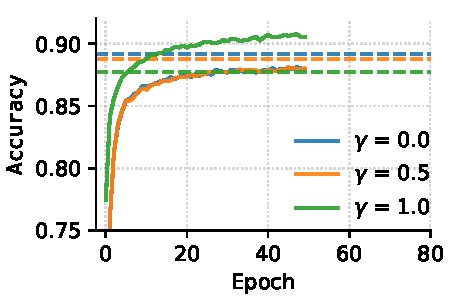
\includegraphics[width=\linewidth]{chapters/ch7_figures/ablation-gamma.pdf}
  \end{center}
  \vspace{-1.5em}
  \caption{Performance of $\gamma$ values.\label{fig:stochastic-projection}}
\end{wrapfigure}
%
Empirically, we find the stochastic extension essential to training models successfully.
In \Cref{fig:stochastic-projection}, we show the accuracy curves over training of a small CNN classifier on Fashion MNIST, with dashed horizontal lines indicating performance on test data.
The experiment evaluates values of $\gamma$: no noise ($\gamma = 1.0$), only noise ($\gamma = 0.0$), and an in-between choice ($\gamma = 0.5$), as per \Cref{eq:altproj-process}.
The model without noise quickly achieves the highest training accuracy, but its dependency on the projected samples, which change only once per epoch, leads to a poorer approximate posterior and generalization.

\subsection{Post-hoc variational inference or full model fitting?}
\label{sec:posthoc-sigmas}
%
\begin{wrapfigure}[10]{r}{0.37\textwidth}
  \vspace{-2em}
  \begin{center}
    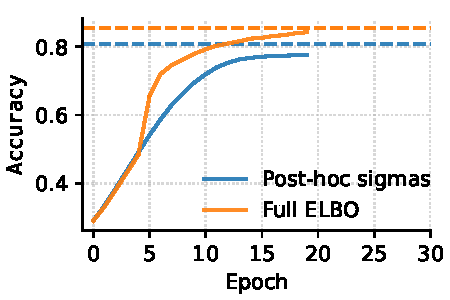
\includegraphics[width=\linewidth]{chapters/ch7_figures/ablation-sigmas.pdf}
  \end{center}
  \vspace{-1.5em}
  \caption{Post-hoc tuning $\sigma_{\ker}, \sigma_{\im}$.\label{fig:posthoc-sigmas}}
\end{wrapfigure}
%
Given the computational effort to evaluate and run the ELBO, it is important to question whether this could be avoided entirely.
One possibility is to start from a well-performing model, and only use the ELBO to tune the variational parameters $\sigma_{\ker}$ and $\sigma_{\im}$, i.e., post-hoc variational inference with a fixed model.
This can be efficiently implemented as we only need to project one set of samples, which can be reused throughout optimization.
With the same experimental setting from before, \Cref{fig:posthoc-sigmas} shows the behavior of such a training procedure.
Interestingly, post-hoc tuning is not \emph{per se} problematic and indeed leads to a well-performing model.
However, the figure shows that optimizing the variational mean with the ELBO improves upon the post-hoc approach.

\paragraph{Warming up as a shortcut.}
\begin{wrapfigure}[10]{r}{0.37\textwidth}
  \vspace{-1.0em}
  \begin{center}
    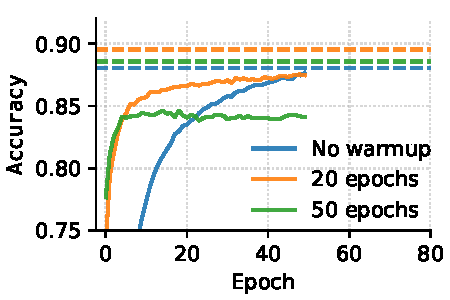
\includegraphics[width=\linewidth]{chapters/ch7_figures/ablation-warmup.pdf}
  \end{center}
  \vspace{-1.5em}
  \caption{Warmup by pretraining.\label{fig:ablation-warmup}}
\end{wrapfigure}
As observed, we can still obtain a well-behaved model from the post-hoc tuning procedure.
Naturally, this informally suggests another way to save computational effort, resources, and time: ``warming up'' the model, first with regular maximum likelihood estimation (or through a pretrained model), and then continuing with ELBO optimization.
We test this hypothesis experimentally, comparing a model trained from scratch using our ELBO and one that starts with a model first fitted using maximum likelihood (\Cref{fig:ablation-warmup}).
Our findings are twofold: (i) warmup using maximum likelihood is an effective way to quickstart the ELBO learning process with the ELBO;
(ii) there is a sweet spot where full convergence of a model on maximum likelihood can lead to the ELBO optimization getting stuck.
We conjecture that this behavior is due to the sharpness of some minima, which negatively affects the evaluation of the expectation term, as it attempts to sample regions of the weight space around the current model weights, which could have drastically different performance, negatively affecting optimization.

\section{Experiments}
\label{sec:experiments}
We evaluate VIKING against popular Bayesian deep learning methods using standard benchmarks for Bayesian deep learning.
Aiming to maintain consistency and simplify comparisons, we adopt the loss-Jacobian (see \Cref{sec:kernel-projections}) when using our proposed variational family.

\paragraph{Toy (sinusoid) regression.}
We first illustrate posterior samples in a 1D regression in \Cref{fig:ivon-vs-viking}.
We train the same model with both IVON \citep{shen2024variational} and VIKING.
While IVON obtains a good model fit, its posterior samples are uninformative with respect to uncertainties.
On the other hand, VIKING shows higher variance close to the boundary of data and beyond, where the model should be less confident.

\begin{figure}[t]
    \centering
    \begin{minipage}{0.5\linewidth}
      \centering
      \hspace{0.15\linewidth}
      \scriptsize{IVON \citep{shen2024variational}}
    \end{minipage}\begin{minipage}{0.5\linewidth}
      \centering
      \hspace{0.05\linewidth}
      \scriptsize{VIKING (ours)}
    \end{minipage}
    \\
    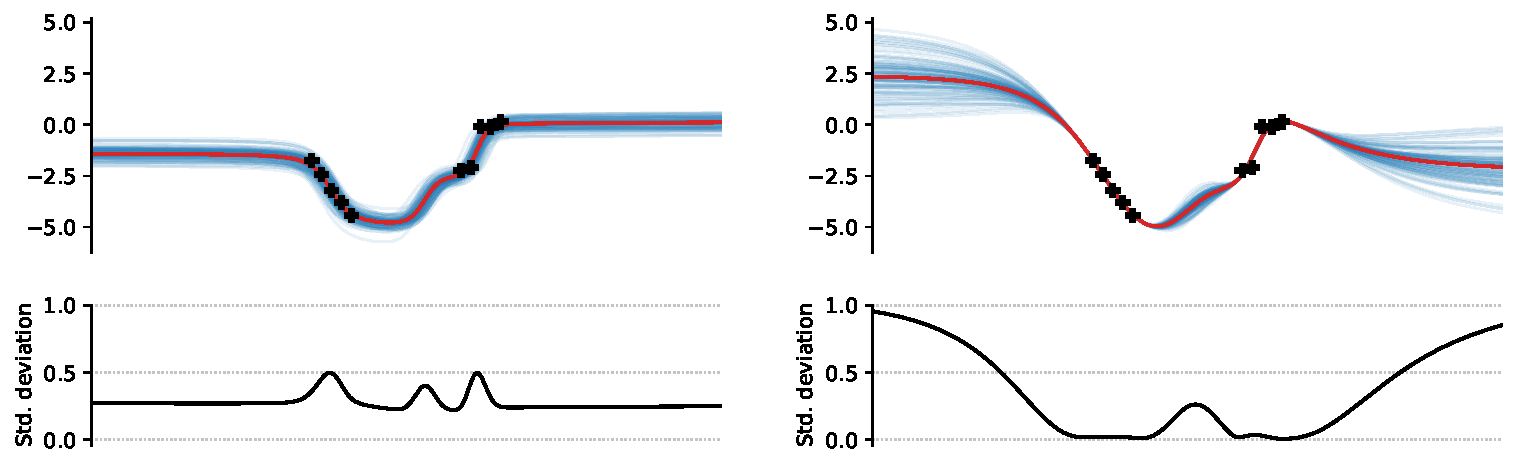
\includegraphics[width=0.9\linewidth]{chapters/ch7_figures/sinusoid.pdf}
    \vspace{-1em}
    \caption{
        A toy regression example on a sinusoid curve with 10 data points.
        \emph{Top:} The curves show the training points in black, with the mean fit as a red line and 100 posterior predictive samples as blue lines.
        \emph{Bottom:} The standard deviation of the predictions over each point in the horizontal axis.
    }
    \label{fig:ivon-vs-viking}
\end{figure}

\paragraph{Image classification.}
Using standard benchmarks, we evaluate our method against the \emph{maximum a posteriori} (MAP) estimate, the (loss-projected) post-hoc method from \citet{miani2025bayes}, IVON \citep{shen2024variational}, SWAG \citep{maddox2019simple}, and a last-layer Laplace approximation.
On MNIST \citep{lecun2010mnist} and Fashion MNIST \citep{xiao2017fashion}, we train a LeNet \citep{lecun1989backpropagation} model, while on SVHN \citep{netzer2011reading} and CIFAR-10 \citep{krizhevsky2009learning} we use a small ResNet \citep{he2016deep}.
The models are compared using accuracy, negative log-likelihood (NLL), expected calibration error (ECE), and maximum calibration error (MCE) \citep{naeini2015obtaining}.

The results in \Cref{tab:in-distribution} show that our ELBO generalize better in most cases, which we hypothesize is due to the interaction between evaluations of the expectation term which constantly ``explores'' the weight space around the current mode through the sampling mechanism, whereas the kernel and image variances that allow this exploration are kept in check by the KL term.
On calibration metrics, our method is particularly effective against the baselines on the SVHN and CIFAR-10 datasets, where the overparametrization of the model (around 220k parameters) is more prominent.
Additional results including deep ensembles and SGLD \citep{welling2011bayesian} are in \Cref{app:experiments-extra}.

\paragraph{Does it scale to larger models?}
To evaluate the scalability of our approach, we also train a ResNet34 (21.7 million parameters) on Imagenette \citep{howard2019imagenette} using VIKING and IVON.
We predominantly aim to demonstrate that VIKING scales to contemporary models despite learning a fully correlated covariance.
The results show a superior performance of our ELBO-trained model, but inferior calibration metrics compared to IVON (\Cref{tab:in-distribution}).

\begin{table}[t]
    \centering
    \caption{
        Experimental results over three runs (mean and standard deviation) on in-distribution test data.
        MAP is a point (model) estimate.
        VIKING and the post-hoc method from \citet{miani2025bayes} use the loss-projected variant.
    }
    \label{tab:in-distribution}
    \resizebox{0.85\textwidth}{!}{%
    \begin{tabular}{crccccc}
    \hline
        & & Accuracy$^\uparrow$
        & Conf.$^\uparrow$
        & NLL$^\downarrow$
        & ECE$^\downarrow$
        & MCE$^\downarrow$ \\
    \hline
        \multirow{6}{*}{\rotatebox[origin=c]{90}{MNIST}}
        & MAP
        & 0.986 \stddev{0.001} & \textbf{0.996 \stddev{0.000}} & 0.070 \stddev{0.005} & 0.247 \stddev{0.011} & 0.861 \stddev{0.045} \\
        & VIKING (ours)
        & \textbf{0.991 \stddev{0.001}} & 0.992 \stddev{0.000} & 0.055 \stddev{0.003} & 0.096 \stddev{0.004} & 0.690 \stddev{0.102} \\
        & \citet{miani2025bayes}
        & 0.949 \stddev{0.000} & 0.813 \stddev{0.018} & 1.225 \stddev{0.099} & 0.666 \stddev{0.007} & 0.894 \stddev{0.011} \\
        & IVON %\cite{shen2024variational}
        & 0.989 \stddev{0.001} & 0.990 \stddev{0.001} & \textbf{0.043 \stddev{0.002}} & \textbf{0.077 \stddev{0.005}} & \textbf{0.651 \stddev{0.042}} \\
        & SWAG %\cite{}
        & 0.982 \stddev{0.000} & 0.982 \stddev{0.001} & 0.064 \stddev{0.006} & 0.788 \stddev{0.005} & 0.906 \stddev{0.013} \\
        & Last Layer LA
        & 0.975 \stddev{0.002} & 0.977 \stddev{0.002} & 0.090 \stddev{0.005} & 0.784 \stddev{0.007} & 0.887 \stddev{0.008} \\
    \hline
        \multirow{6}{*}{\rotatebox[origin=c]{90}{Fashion MNIST}}
        & MAP
        & 0.883 \stddev{0.002} & \textbf{0.942 \stddev{0.003}} & 0.410 \stddev{0.010} & 0.153 \stddev{0.008} & \textbf{0.590 \stddev{0.141}} \\
        & VIKING (ours)
        & \textbf{0.900 \stddev{0.001}} & 0.928 \stddev{0.001} & 0.332 \stddev{0.003} & 0.075 \stddev{0.002} & 0.611 \stddev{0.160} \\
        & \citet{miani2025bayes}
        & 0.871 \stddev{0.006} & 0.744 \stddev{0.031} & 1.529 \stddev{0.371} & 0.617 \stddev{0.025} & 0.901 \stddev{0.013} \\
        & IVON %\cite{}
        & 0.897 \stddev{0.004} & 0.926 \stddev{0.001} & 0.335 \stddev{0.011} & \textbf{0.073 \stddev{0.005}} & 0.683 \stddev{0.024} \\
        & SWAG %\cite{}
        & 0.898 \stddev{0.001} & 0.931 \stddev{0.006} & \textbf{0.327 \stddev{0.001}} & 0.725 \stddev{0.003} & 0.907 \stddev{0.003} \\
        & Last Layer LA
        & 0.896 \stddev{0.002} & 0.931 \stddev{0.005} & 0.339 \stddev{0.011} & 0.727 \stddev{0.004} & 0.902 \stddev{0.004} \\
    \hline
        \multirow{6}{*}{\rotatebox[origin=c]{90}{SVHN}}
        & MAP
        & 0.947 \stddev{0.004} & 0.963 \stddev{0.004} & 0.201 \stddev{0.014} & 0.055 \stddev{0.010} & 0.608 \stddev{0.228} \\
        & VIKING (ours)
        & \textbf{0.960 \stddev{0.001}} & \textbf{0.964 \stddev{0.001}} & \textbf{0.177 \stddev{0.002}} & \textbf{0.028 \stddev{0.002}} & \textbf{0.308 \stddev{0.024}} \\
        & \citet{miani2025bayes}
        & 0.949 \stddev{0.003} & 0.948 \stddev{0.005} & 0.191 \stddev{0.007} & 0.734 \stddev{0.017} & 0.880 \stddev{0.012} \\
        & IVON %\cite{}
        & 0.943 \stddev{0.002} & 0.888 \stddev{0.007} & 0.302 \stddev{0.016} & 0.082 \stddev{0.004} & 0.492 \stddev{0.248} \\
        & SWAG %\cite{}
        & 0.947 \stddev{0.004} & 0.897 \stddev{0.007} & 0.217 \stddev{0.014} & 0.745 \stddev{0.007} & 0.874 \stddev{0.003} \\
        & Last Layer LA
        & 0.946 \stddev{0.001} & 0.943 \stddev{0.005} & 0.197 \stddev{0.009} & 0.740 \stddev{0.007} & 0.899 \stddev{0.009} \\
    \hline
        \multirow{6}{*}{\rotatebox[origin=c]{90}{CIFAR-10}}
        & MAP
        & 0.824 \stddev{0.012} & 0.869 \stddev{0.003} & 0.536 \stddev{0.055} & 0.075 \stddev{0.012} & 0.619 \stddev{0.243} \\
        & VIKING (ours)
        & 0.877 \stddev{0.004} & 0.893 \stddev{0.003} & 0.407 \stddev{0.010} & \textbf{0.041 \stddev{0.004}} & \textbf{0.331 \stddev{0.094}} \\
        & \citet{miani2025bayes}
        & 0.855 \stddev{0.002} & 0.701 \stddev{0.013} & 2.643 \stddev{0.205} & 0.559 \stddev{0.006} & 0.802 \stddev{0.005} \\
        & IVON %\cite{}
        & 0.835 \stddev{0.017} & 0.763 \stddev{0.005} & 0.817 \stddev{0.075} & 0.086 \stddev{0.014} & 0.436 \stddev{0.244} \\
        & SWAG %\cite{}
        & 0.865 \stddev{0.029} & 0.914 \stddev{0.035} & 0.445 \stddev{0.063} & 0.694 \stddev{0.018} & 0.881 \stddev{0.005} \\
        & Last Layer LA
        & \textbf{0.894 \stddev{0.001}} & \textbf{0.944 \stddev{0.001}} & \textbf{0.406 \stddev{0.005}} & 0.704 \stddev{0.000} & 0.880 \stddev{0.007} \\
    \hline
        \multirow{2}{*}{\rotatebox[origin=c]{90}{Imagenette\hspace{-2mm}}}
        & MAP
        & 0.852 \stddev{0.002} & 0.883 \stddev{0.007} & 0.481 \stddev{0.009} & 0.084 \stddev{0.010} & 0.717 \stddev{0.082} \\
        & VIKING (ours)
        & \textbf{0.887 \stddev{0.003}}& \textbf{0.906 \stddev{0.002}} & \textbf{0.403 \stddev{0.010}} & 0.077 \stddev{0.001} & 0.612 \stddev{0.162} \\
        & IVON %\cite{}
        & 0.876 \stddev{0.023} & 0.849 \stddev{0.013} & 0.656 \stddev{0.136} & \textbf{0.069 \stddev{0.011}} & \textbf{0.464 \stddev{0.230}} \\
    \hline
    \end{tabular} }
\end{table}

\paragraph{Out-of-distribution detection.}
Next, we evaluate VIKING in out-of-distribution (OOD) detection tasks.
We use the maximum variance of the softmax probabilities across output dimensions as an OOD score for both IVON and VIKING.
In addition to the datasets from before, we use EMNIST and CIFAR-100 as OOD data.
For ease of comparison, our experimental setup replicates that of \citet{miani2025bayes}, so we additionally use their reported numbers for the other baselines as well.
\Cref{tab:out-of-distribution} summarizes the obtained results.
At a glance, VIKING performs on par with the best models, sometimes overperforming the other baselines by a big margin (e.g., MNIST $\rightarrow$ FMNIST and KMNIST) and other times being a close second.
Overall, this further confirms the empirical performance of our variational family and ELBO optimization in obtaining robust models.

\begin{table}[t]
    \caption{
        Area under ROC ($\uparrow$) performance on out-of-distribution detection.
        VIKING and the post-hoc method from \citet{miani2025bayes} use the loss-projected variant.
    }
    \label{tab:out-of-distribution}
    \hspace{2.7em}
    \resizebox{0.88\textwidth}{!}{%
    \begin{tabular}{rcccccc}
    \hline
        \textbf{In-dist.}
        & \multicolumn{3}{c}{\textbf{MNIST}}
        & \multicolumn{3}{c}{\textbf{FMNIST}} \\
        \cline{2-4} \cline{5-7}
        \textbf{Out-of-dist.}
        & FMNIST & KMNIST & EMNIST
        & MNIST & KMNIST & EMNIST \\
    \hline
        MAP
        & 0.928 \stddev{0.015} & 0.934 \stddev{0.004} & 0.890 \stddev{0.002}
        & 0.728 \stddev{0.048} & 0.791 \stddev{0.014} & 0.659 \stddev{0.035} \\
        VIKING (ours)
        & \textbf{0.972 \stddev{0.003}} & \textbf{0.965 \stddev{0.002}} & 0.913 \stddev{0.006}
        & 0.898 \stddev{0.025} & \textbf{0.926 \stddev{0.002}} & 0.830 \stddev{0.020} \\
        \citet{miani2025bayes}
        & 0.899 \stddev{0.011} & 0.856 \stddev{0.002} & 0.893 \stddev{0.006}
        & \textbf{0.914 \stddev{0.035}} & 0.907 \stddev{0.026} & \textbf{0.928} \stddev{0.007} \\
        IVON %\cite{}
        & 0.948 \stddev{0.004} & 0.945 \stddev{0.007} & \textbf{0.918 \stddev{0.008}}
        & 0.801 \stddev{0.020} & 0.867 \stddev{0.005} & 0.739 \stddev{0.025} \\
        SWAG %\cite{}
        & 0.917 \stddev{0.024} & 0.861 \stddev{0.032} & 0.916 \stddev{0.010}
        & 0.685 \stddev{0.014} & 0.655 \stddev{0.015} & 0.751 \stddev{0.032} \\
        Last Layer LA
        & 0.793 \stddev{0.215} & 0.759 \stddev{0.166} & 0.782 \stddev{0.182}
        & 0.768 \stddev{0.001} & 0.699 \stddev{0.020} & 0.824 \stddev{0.016} \\
    \hline
    \end{tabular}}

    \vspace{0.3cm}
    \hspace{2.7em}
    \resizebox{0.67\textwidth}{!}{%
    \noindent
    \begin{tabular}{rcccc}
    \hline
        \textbf{In-dist.}
        & \multicolumn{2}{c}{\textbf{SVHN}}
        & \multicolumn{2}{c}{\textbf{CIFAR-10}} \\
        \cline{2-3} \cline{4-5}
        \textbf{Out-of-dist.}
        & CIFAR-10 & CIFAR-100
        & SVHN & CIFAR-100 \\
    \hline
        MAP
        & 0.946 \stddev{0.006} & 0.941 \stddev{0.007}
        & 0.831 \stddev{0.019} & 0.778 \stddev{0.013} \\
        VIKING (ours)
        & 0.947 \stddev{0.002} & 0.943 \stddev{0.002}
        & 0.827 \stddev{0.007} & \textbf{0.805 \stddev{0.003}} \\
        \citet{miani2025bayes}
        & \textbf{0.966 \stddev{0.009}} & \textbf{0.960 \stddev{0.006}}
        & \textbf{0.863 \stddev{0.008}} & 0.800 \stddev{0.013} \\
        IVON %\cite{}
        & 0.822 \stddev{0.014} & 0.826 \stddev{0.009}
        & 0.648 \stddev{0.019} & 0.714 \stddev{0.012} \\
        SWAG %\cite{}
        & 0.777 \stddev{0.029} & 0.787 \stddev{0.027}
        & 0.798 \stddev{0.040} & 0.782 \stddev{0.042} \\
        Last Layer LA
        & 0.914 \stddev{0.005} & 0.908 \stddev{0.005}
        & 0.811 \stddev{0.024} & 0.801 \stddev{0.026} \\
    \hline
    \end{tabular}}
    
\end{table}

\paragraph{Generative modelling.}
Finally, we demonstrate our approach applied to generative modelling.
We train a variational autoencoder (VAE, \citet{kingma2013auto}) until convergence. From that starting point, we further refine the decoder's 1.6 million parameters using both IVON and VIKING.
We draw 32 samples from each of the resulting approximate decoder posteriors, which we use to both reconstruct images and measure uncertainties.
\Cref{fig:celeba-samples} displays the reconstructed samples and the variance across the posterior samples per reconstructed image.
Overall, both posteriors qualitatively recover well-performing models.
The methods discern themselves more prominently upon inspection of the variances across the reconstructions of the different posterior samples.
Notably, IVON tends to capture variance across all features of the image, including the background.
VIKING focuses the variance on facial features and outline instead, showing a disregard for the less-relevant aspects of the data.
To assess the model uncertainties, we compute the median value of the standard deviations per pixel produced by each of the 16k generated samples and summarize their distribution in \Cref{fig:gen_ood_in_hist}.
Our in-distribution samples come from a standard Gaussian sample, whereas out-of-distribution samples come from a Gaussian with twice the variance.
The uncertainties produced by VIKING show well-separated distributions clearly detecting OOD samples, while IVON does not.

\begin{figure}
    \centering
    {\setlength{\tabcolsep}{0.1em}
    \begin{tabular}{rcc}
    & Reconstructions
    & Variances across channels
    \\
    \rotatebox{90}{\hspace{1em} ~~~~VIKING (ours)}
    & 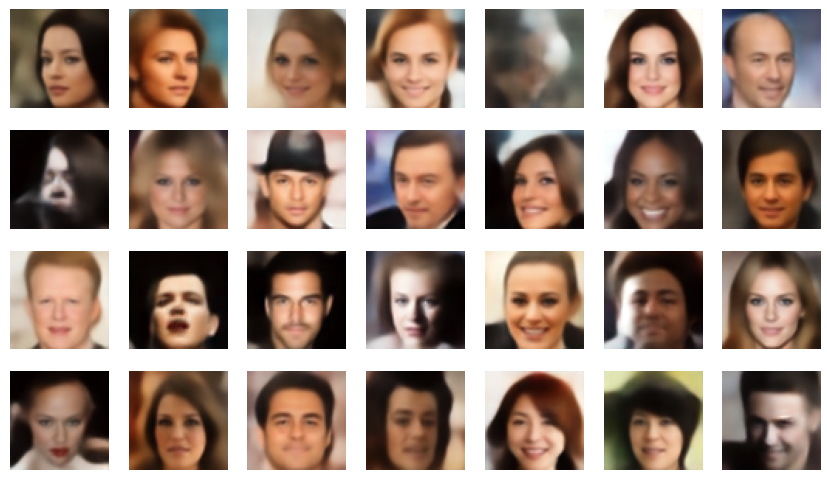
\includegraphics[width=0.475\linewidth]{chapters/ch7_figures/elbo_reconstructions_kivi.png}
    & 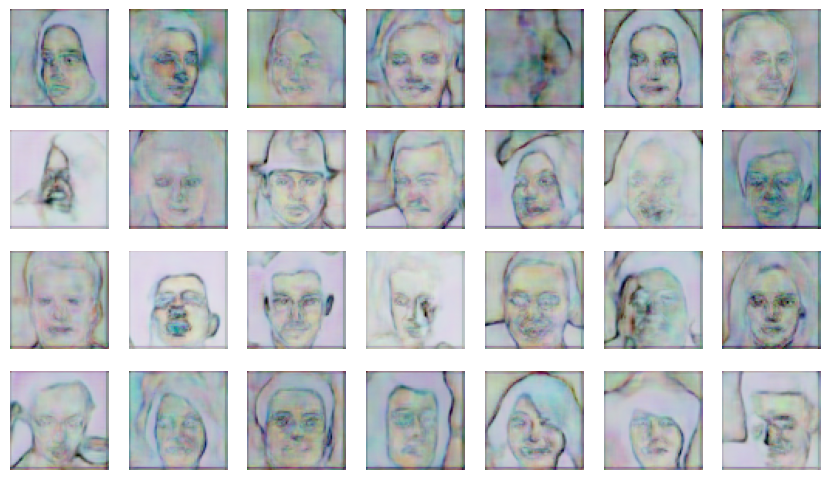
\includegraphics[width=0.475\linewidth]{chapters/ch7_figures/uncertainty_kivi_rgb_inverse.png}
    \\
    & & \\
    \rotatebox{90}{\hspace{4.5em} IVON~~~~~~~~}
    & 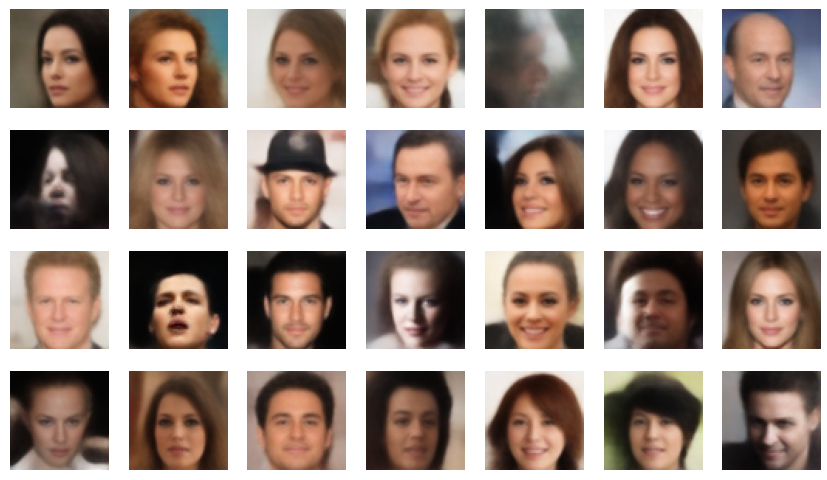
\includegraphics[width=0.475\linewidth]{chapters/ch7_figures/mle_reconstructions_ivon.png}
    & 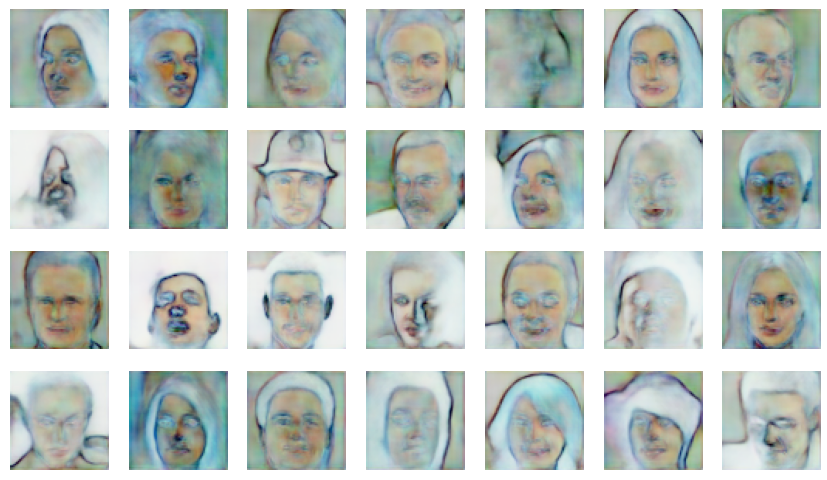
\includegraphics[width=0.475\linewidth]{chapters/ch7_figures/uncertainty_rgb_inverse_ivon.png}
    \end{tabular}}
    \vspace{-0.5em}
    \caption{
        Reconstructed samples taken from the latent space prior of variational autoencoders trained with IVON and VIKING.
        Using 32 posterior samples, the posterior variances compare key semantic features, such as contours between foreground and background, and eyes.
    }
    \label{fig:celeba-samples}
\end{figure}

\begin{figure}
    \centering
    {\setlength{\tabcolsep}{0.1em}
    \begin{tabular}{rcc}
    & {\small IVON}
    & {\small VIKING}
    \\
    &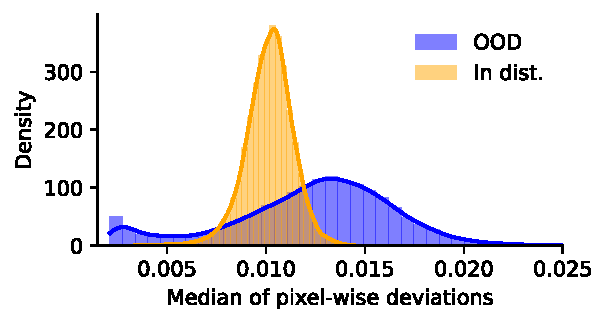
\includegraphics[width=0.45\linewidth]{chapters/ch7_figures/ivon_median.pdf}
    & 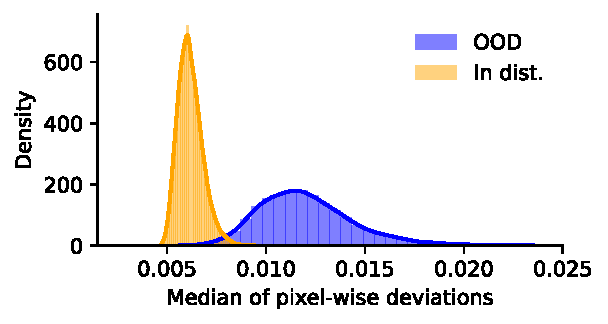
\includegraphics[width=0.45\linewidth]{chapters/ch7_figures/viking_median.pdf}
    \end{tabular}}
    \vspace{-1em}
    \caption{
        Histograms of uncertainties on 16K in- and out-of-distribution latent samples according to IVON and VIKING.
        Uncertainties are computed as median of pixel-wise standard deviations computed by decoding the latent sample using 32  posterior model samples.
    }
    \label{fig:gen_ood_in_hist}
\end{figure}